\documentclass[12pt,a4paper]{article}
\usepackage[utf8]{inputenc}
\usepackage{amsmath}
\usepackage{amsfonts}
\usepackage{amssymb}
\usepackage[spanish]{babel}
\usepackage{graphicx}
\pagestyle{headings}
\author{Juan Sebastian Gonzalez Camacho (1968220)}
\title{Requirements_Specification}
\begin{document}
\begin{titlepage}
\centering
{
\includegraphics[width=0.18 \textwidth]{IMAGES/logo.png} \par}
\vfill
{\bfseries\LARGE Universidad del Valle\par}
{\Large Sede Tuluá\par}
\vfill
{\scshape\Large Ingeniería de Sistemas \par}
\vfill
{\scshape\Huge Borvo-Medicinae Operam \par}
\vfill
{\itshape\Large Proyecto Final de Bases de Datos y Desarrollo de Software I \par}
\vfill
{\Large Autores: \par}
{\Large Juan Sebastian González Camacho - 1968220 \par}
{\Large Carlos Alberto Delgado Galeano - 1968127 \par}
{\Large Jesús Alberto Gil Ayala - 1968231 \par}
{\Large Andrés Felipe Ruíz Buriticá - 1968171 \par}
{\Large Jhoan Sebastian Rojas Holguin - 1958337 \par}
\vfill
{\Large 9 de Octubre del 2022 \par}
\end{titlepage}
\tableofcontents
\newpage
\section{Introducción}
Esta es la Especificación de Requisitos de Software para \emph{Borvo-Medicinae Operam}, un producto de software encargado de la gestión de información de la EPS ``Esperar para Salvarse''. Este documento ha sido elaborado a partir del estándar \textit{IEEE 830}.
\subsection{Propósito}
Definir y presentar de forma ordenada los requisitos y especificaciones que deberá cumplir el software \emph{Borvo-Medicinae Operam}, que elaboraremos para la EPS ``Esperar para Salvarse'', el cual permitirá gestionar la información de cotizantes, beneficiarios e instituciones externas asociadas a ella.
\subsection{Ámbitos del Sistema}
Con \emph{Borvo-Medicinae Operam} buscamos desarrollar un software web que sirva para mejorar los procesos y subprocesos de la EPS, con tal de fortalecer la gestión de la información de sus cotizantes, beneficiarios y las IPS asociadas para brindar un servicio oportuno.\\

Los usuarios tienen diferentes funciones según su rol: los administradores podrán gestionar afiliados, empresas, IPS, contratos, órdenes de servicio y generar reporte de afiliados por estado, órdenes por paciente y afiliados por empresa, los trabajadores pueden consultar su propia información y el banco puede cargar la información de los pagos que reportan las empresas, los cuales pueden hacerse individualmente o cargarse en bloque desde archivos.
\subsection{Definiciones, Acrónimos y Abreviaturas}
\begin{itemize}
\item \textbf{EPS:} Entidad Promotora de Salud.
\item \textbf{IPS:} Institución Prestadora de Salud.
\item \textbf{GUI:} Interfaz Gráfica de Usuario.
\item \textbf{IDE:} Entorno Integrado de Desarrollo.
\item \textbf{SGBD} Sistema de Gestión de Bases de Datos.
\item \textbf{HTML:} Lenguaje de Marcas de Hipertexto.
\item \textbf{MER:} Modelo Entidad - Relación.
\item \textbf{UML:} Lenguaje Unificado de Modelado.
\item \textbf{Software:} Conjunto de programas y rutinas que permiten a la computadora realizar determinadas tareas.
\item \textbf{Front-end:} Es la parte de una aplicación que interactúa con los usuarios, es conocida como el lado del cliente. Básicamente es todo lo que vemos en la pantalla cuando accedemos a un sitio web o aplicación: tipos de letra, colores, adaptación para distintas pantallas, los efectos del ratón, teclado, movimientos, desplazamientos, efectos visuales… y otros elementos que permiten navegar dentro de una página web. Este conjunto crea la experiencia del usuario.
\item \textbf{Back-end:} Es la parte del desarrollo web que se encarga de que toda la lógica de una página web  funcione. Se trata del conjunto de acciones que pasan en una web pero que no vemos como, por ejemplo, la comunicación con el servidor.
\item \textbf{JavaScript:} Es un lenguaje de programación interpretado, dialecto del estándar ECMAScript. Se define como orientado a objetos, basado en prototipos, imperativo, débilmente tipado y dimámico.
\item Aquí se van agregando otras abreviaturas, acrónimos y definiciones.
\end{itemize}
\subsection{Referencias}
\begin{itemize}
\item Especificación de Requisitos según el estándar de IEEE 830.
\end{itemize}
\subsection{Visión General del Documento}
Este documento contiene la descripción del software, sus requerimientos funcionales y no funcionales, casos de uso y escenarios, el diseño de la interfaz, la arquitectura, el modelo de la base de datos y la implementación.
\section{Descripción General}
La aplicación web \emph{Borvo-Medicinae Operam} es un software integrado que maneja la información y las actividades de la Entidad Promotora de Salud de forma digital para una administración más eficaz, con mejor rendimiento y mayor confiabilidad. A partir de tecnologías de vanguardia que implementan interfaces claras e intuitivas, se facilita la gestión de los detalles del paciente, la información administrativa, médica y financiera del centro de salud.
\subsection{Perspectiva del Producto}
\emph{Borvo-Medicinae Operam} está planeado como un software independiente, que no requiere sistemas externos para su funcionamiento e interacción. 
\subsection{Funciones del Producto}
\vspace{5mm}
\begin{figure}[h]
{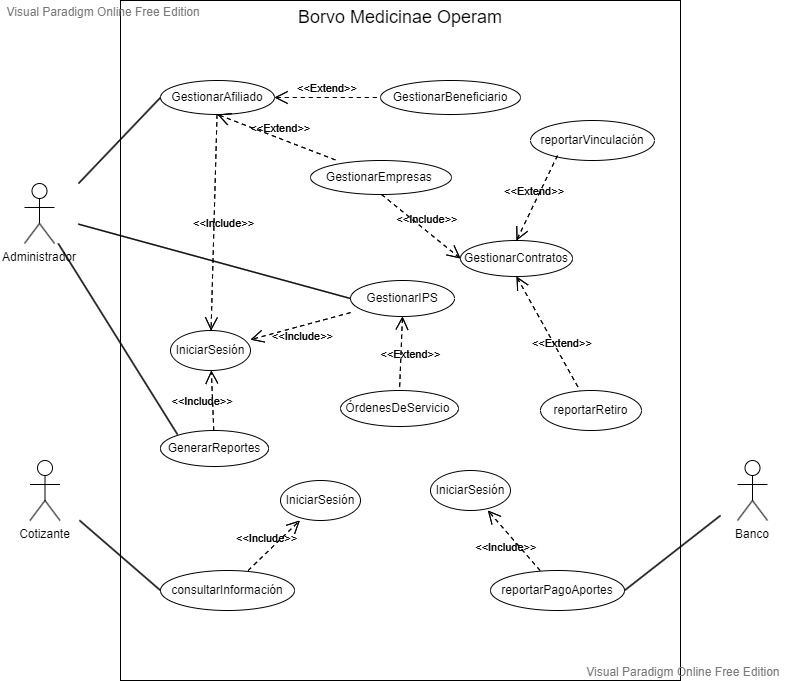
\includegraphics[width=1 \textwidth]{IMAGES/use_cases_diagram.png} \par}
\caption{Diagrama de Casos de Uso.}
\end{figure}
\subsection{Características de los Usuarios}
\begin{center}
\begin{tabular}{|p{3.5cm}| p{11.5cm}|}
\hline 
\multicolumn{2}{|c|}{\textbf{Administrador}} \\ 
\hline 
\textbf{Nivel Educativo} & Educación superior / Especialista en TICs.\\ 
\hline 
\textbf{Experiencia} & Manejo de TICs y gestión de sistemas de información. \\ 
\hline 
\textbf{Actividades} & Gestionar afiliados, empresas IPS, contratos, órdenes de servicio y generar reporte de afiliados por estado, órdenes por paciente y afiliados por empresa. \\ 
\hline 
\end{tabular}
\vspace{5mm}

\begin{tabular}{|p{3.5cm}| p{11.5cm}|}
\hline 
\multicolumn{2}{|c|}{\textbf{Trabajador}} \\ 
\hline 
\textbf{Nivel Educativo} & Educación secundaria.\\ 
\hline 
\textbf{Experiencia} & Manejo de TICs.\\ 
\hline 
\textbf{Actividades} & Consultar su propia información.\\ 
\hline 
\end{tabular}
\vspace{5mm}

\begin{tabular}{|p{3.5cm}| p{11.5cm}|}
\hline 
\multicolumn{2}{|c|}{\textbf{Banco}} \\ 
\hline 
\textbf{Nivel Educativo} & Educación superior / Especialista en TICs.\\ 
\hline 
\textbf{Experiencia} & Gestión de sistemas de información.\\ 
\hline 
\textbf{Actividades} & Puede cargar la información de los pagos que reportan las empresas, los cuales pueden hacerse individualmente o cargarse en bloque desde archivos.\\ 
\hline 
\end{tabular}
\vspace{5mm}
\end{center}
\subsection{Restricciones}
\begin{itemize}
\item El software requiere conexión a internet para su funcionamiento.
\item El software debe contar con un sistema de login de sesión.
\item Todo usuario Administrador debe tener noción de la gestión de la EPS.
\item El software debe funcionar las 24 horas del día, los 7 días de la semana.
\item El software debe ser accesible desde cualquier dispositivo.
\item Aquí se van añadiendo restricciones a medida que se va desarrollando el software (p.ej uso de algun framework en especifico, de alguna API, tipo de aplicación, etc).
\end{itemize}
\subsection{Suposiciones y Dependencias}
\begin{itemize}
\item Los equipos en donde se utilice el software deben contar con un mínimo de recursos, navegador y una buena conexión a Internet.
\end{itemize}
\subsection{Requisitos Futuros}
Texto
\section{Requisitos Específicos}
\subsection{Interfaces Externas}
\begin{center}
\begin{tabular}{|p{5.5cm}| p{9.5cm}|}
\hline 
\multicolumn{2}{|c|}{\textbf{Nombre del Requisito}}\\ 
\hline 
\textbf{Descripción} & • \\ 
\hline 
\textbf{Pre-condición} & • \\ 
\hline 
\textbf{Flujo de Eventos} & • \\ 
\hline 
\textbf{Flujo Alterno} & • \\ 
\hline 
\textbf{Post-condición}  & • \\ 
\hline 
\textbf{Requisitos No Funcionales} & • \\ 
\hline 
\end{tabular}
\vspace{5mm}

\begin{tabular}{|p{5.5cm}| p{9.5cm}|}
\hline 
\multicolumn{2}{|c|}{\textbf{Nombre del Requisito}}\\ 
\hline 
\textbf{Descripción} & • \\ 
\hline 
\textbf{Pre-condición} & • \\ 
\hline 
\textbf{Flujo de Eventos} & • \\ 
\hline 
\textbf{Flujo Alterno} & • \\ 
\hline 
\textbf{Post-condición}  & • \\ 
\hline 
\textbf{Requisitos No Funcionales} & • \\ 
\hline 
\end{tabular}
\vspace{5mm}

\begin{tabular}{|p{5.5cm}| p{9.5cm}|}
\hline 
\multicolumn{2}{|c|}{\textbf{Nombre del Requisito}}\\ 
\hline 
\textbf{Descripción} & • \\ 
\hline 
\textbf{Pre-condición} & • \\ 
\hline 
\textbf{Flujo de Eventos} & • \\ 
\hline 
\textbf{Flujo Alterno} & • \\ 
\hline 
\textbf{Post-condición}  & • \\ 
\hline 
\textbf{Requisitos No Funcionales} & • \\ 
\hline 
\end{tabular}
\vspace{5mm}

\begin{tabular}{|p{5.5cm}| p{9.5cm}|}
\hline 
\multicolumn{2}{|c|}{\textbf{Nombre del Requisito}}\\ 
\hline 
\textbf{Descripción} & • \\ 
\hline 
\textbf{Pre-condición} & • \\ 
\hline 
\textbf{Flujo de Eventos} & • \\ 
\hline 
\textbf{Flujo Alterno} & • \\ 
\hline 
\textbf{Post-condición}  & • \\ 
\hline 
\textbf{Requisitos No Funcionales} & • \\ 
\hline 
\end{tabular}
\end{center}
\subsection{Funciones}
\subsection{Requisitos de Rendimiento}
\subsection{Restricciones de Diseño}
\subsection{Atributos del Sistema}
\subsection{Otros Requisitos}

\end{document}
